\section{Turtlebot 2}


\begin{figure}[H]
    \centering
    \begin{minipage}[b]{0.56\linewidth}
     Turtlebot 2 is an easy-to-use low-cost robotics platform aimed at research and hobby usage and can be seen on figure \ref{fig:turtlebot2}\cite{turtlebot2Kobuki}. 
     Turtlebot is an open source hardware and the documentation can be found on the webpage for the turtlebot. One of the biggest strengths of the Turtlebot is its worldwide support community\cite{turtlebotworld}. It is controlled with a software called "ROS" which will be further explained in section \ref{sec:ROS}.
     Turtlebot 2 is based on a Kobuki mobile base, which has a variety of sensors such as odometry sensor with a 52 ticks/encoder revolution, a gyroscope, bumper sensor, cliff sensors in addition to two wheel drop sensors. The base has programmable LEDs and buttons as well as power sources. The functional specifications of the base are listed below:
    \end{minipage}
    \hspace{0.3cm}
    \begin{minipage}[b]{0.33\linewidth}
    \centering
    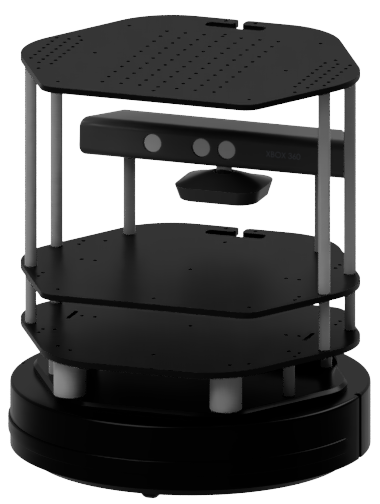
\includegraphics[width=\textwidth]{figures/turtlebot_2.png}
    \caption{CAD model of the Turtlebot 2\cite{TURTLE_build}. The original turtlebot was develop by Melonee Wise and Tully Foote at Willow Garage\cite{TURTLE_devs}.}
    \label{fig:turtlebot2}
    \end{minipage}
\end{figure}
    \begin{itemize}
    	\item Maximum translational and rotational velocity is 70cm/s and 180 deg/s respectively.
    	\item Maximum payload is 5kg on hard floor and 4kg on carpet.
    	\item Does not drive off a cliff with a depth > 5cm.
    	\item Climbs thresholds of up to 12mm.
    	\item Operating time is 3 or 7 hours depending on the battery (small/large).
    	\item Automatic docking within 2m x 5m area in front of the docking station.
    \end{itemize}


The turtlebot enables mounting of different hardware for testing new systems and are therefore well suited for prototyping. As the placement of different components impacts the functionality of the system, the placement of sensors is described in the following.